
\begin{figure}[H]
  {
    \setlength{\tabcolsep}{3.0pt}
    \setlength\cmidrulewidth{\heavyrulewidth} % Make cmidrule = 
    \begin{adjustbox}{height=5cm,center}
      \footnotesize
      \begin{tabular}{ll}

        \makecell[l]{
\icode{.BYTE \$00}\\
\icode{.BYTE \$FF}
} & \makecell[l]{
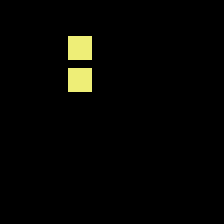
\includegraphics[width=1.3cm]{src/patterns/pixels/pixel_pattern1_0.png}%
} \\
        \midrule

        \makecell[l]{
\icode{.BYTE \$01,\$02}\\
\icode{.BYTE \$FF,\$FE}
} & \makecell[l]{

\includegraphics[width=1.3cm]{src/patterns/pixels/pixel_pattern1_1.png}%
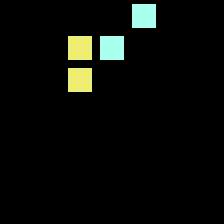
\includegraphics[width=1.3cm]{src/patterns/pixels/pixel_pattern1_2.png}%
} \\
        \midrule

        \makecell[l]{
\icode{.BYTE \$01,\$02,\$03}\\
\icode{.BYTE \$00,\$00,\$00}
} & \makecell[l]{
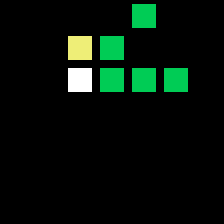
\includegraphics[width=1.3cm]{src/patterns/pixels/pixel_pattern1_3.png}%

\includegraphics[width=1.3cm]{src/patterns/pixels/pixel_pattern1_4.png}%

\includegraphics[width=1.3cm]{src/patterns/pixels/pixel_pattern1_5.png}%
} \\
        \midrule

        \makecell[l]{
\icode{.BYTE \$01,\$02,\$03,\$04}\\
\icode{.BYTE \$01,\$02,\$03,\$04}
} & \makecell[l]{
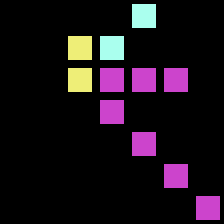
\includegraphics[width=1.3cm]{src/patterns/pixels/pixel_pattern1_6.png}%
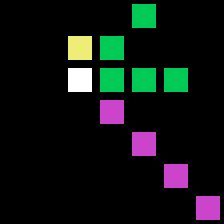
\includegraphics[width=1.3cm]{src/patterns/pixels/pixel_pattern1_7.png}%
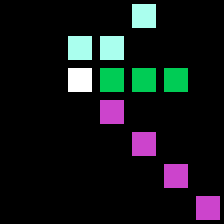
\includegraphics[width=1.3cm]{src/patterns/pixels/pixel_pattern1_8.png}%
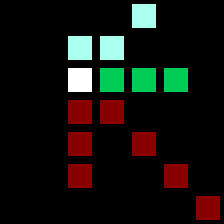
\includegraphics[width=1.3cm]{src/patterns/pixels/pixel_pattern1_9.png}%
} \\
        \midrule

        \makecell[l]{
\icode{.BYTE \$00,\$00,\$00}\\
\icode{.BYTE \$01,\$02,\$03}
} & \makecell[l]{
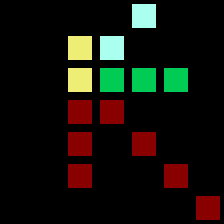
\includegraphics[width=1.3cm]{src/patterns/pixels/pixel_pattern1_10.png}%
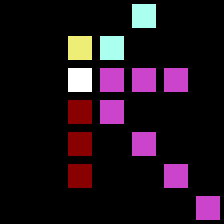
\includegraphics[width=1.3cm]{src/patterns/pixels/pixel_pattern1_11.png}%
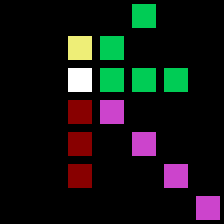
\includegraphics[width=1.3cm]{src/patterns/pixels/pixel_pattern1_12.png}%
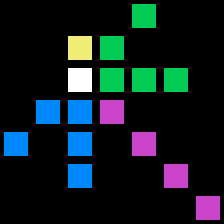
\includegraphics[width=1.3cm]{src/patterns/pixels/pixel_pattern1_13.png}%
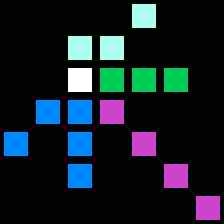
\includegraphics[width=1.3cm]{src/patterns/pixels/pixel_pattern1_14.png}%
} \\
        \midrule

        \makecell[l]{
\icode{.BYTE \$FF,\$FE}\\
\icode{.BYTE \$01,\$02}
} & \makecell[l]{
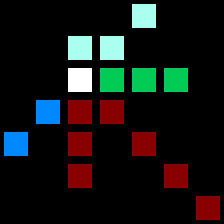
\includegraphics[width=1.3cm]{src/patterns/pixels/pixel_pattern1_15.png}%
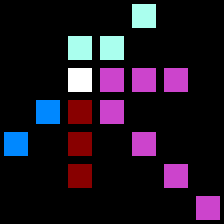
\includegraphics[width=1.3cm]{src/patterns/pixels/pixel_pattern1_16.png}%
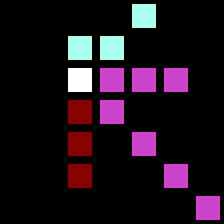
\includegraphics[width=1.3cm]{src/patterns/pixels/pixel_pattern1_17.png}%
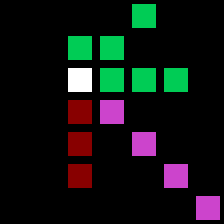
\includegraphics[width=1.3cm]{src/patterns/pixels/pixel_pattern1_18.png}%
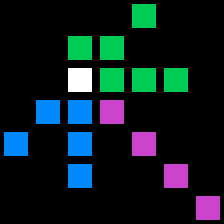
\includegraphics[width=1.3cm]{src/patterns/pixels/pixel_pattern1_19.png}%
} \\
        \midrule

        \makecell[l]{
\icode{.BYTE \$FF}\\
\icode{.BYTE \$00}
} & \makecell[l]{
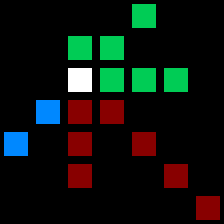
\includegraphics[width=1.3cm]{src/patterns/pixels/pixel_pattern1_20.png}%
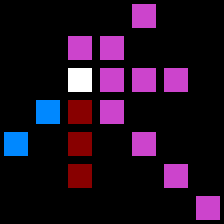
\includegraphics[width=1.3cm]{src/patterns/pixels/pixel_pattern1_21.png}%
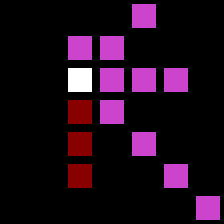
\includegraphics[width=1.3cm]{src/patterns/pixels/pixel_pattern1_22.png}%
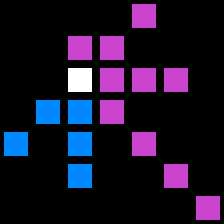
\includegraphics[width=1.3cm]{src/patterns/pixels/pixel_pattern1_23.png}%
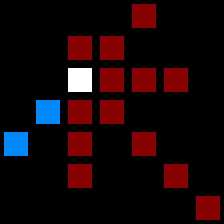
\includegraphics[width=1.3cm]{src/patterns/pixels/pixel_pattern1_24.png}%
} \\
        \midrule

        \makecell[l]{
\icode{.BYTE}\\
\icode{.BYTE}
} & \makecell[l]{
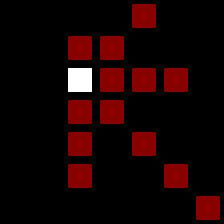
\includegraphics[width=1.3cm]{src/patterns/pixels/pixel_pattern1_25.png}%
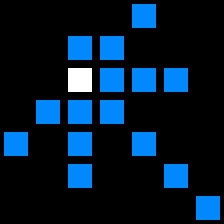
\includegraphics[width=1.3cm]{src/patterns/pixels/pixel_pattern1_26.png}%
} \\
        \midrule

      \end{tabular}
    \end{adjustbox}
  }\caption{The purpose of each of the oscillator values.}
\end{figure}
